\chapter{Experimentation and Analysis\label{ch:Experimentation and Analysis}}

This chapter is intended to provide the experimental proof of the proposed extension of the previously formulated algorithm from \cite{ref5}. Through this chapter, the detailed explanation of the additional constraints that are added to the unoptimized algorithm from the previous chapter is provided. Next micro and macro agent simulations are presented pertaining to certain cases and scenarios to compare between the unoptimized and the optimized algorithms. The resulting observations and statistics are then presented for further analysis and the implications are then discussed.

\section{Optimization through Constraints}
\label{sec: Optimization through Constraints}

From the equations \ref{eq1}, \ref{eq2} and \ref{eq3}, the basic conditions for agent occupancy, flow control and cell capacity is discussed. However these conditions are hardly realistic when compared to modelling a real crowd of agents. In realistic scenarios, groups of people have altered behavior, confusion panic etc. There will be different forms of social constraints, varying movement speeds, and due to the impaired cognition, perceptions can change leading to different decisions that are made during a catastrophe. To model some of these realistic scenarios, it became evident that the inclusion of certain more properties to the scenario was mandatory. The following conditions as mentioned in section \ref{sec:intro:Objectives and Approach} is analyzed here:

\begin{enumerate}
  \item Cell capacity specification by defining social distances
  \begin{itemize}
  	\item Although PedSim comes by default with a cell class, it does not go coherently with the topology, as cell divisions are highly subjective and can change their length and breadth according to the defined scenario. To cater for this, manipulation of the social forces constraint causes agents to maintain a certain "social distance" from each other. This can be used to our advantage to simulate cell capacities based on these social distances.
  \end{itemize}
  \item Definition of total area capacity and doors flow capacity constraints -congestion control
  \begin{itemize}
  	\item The algorithm presented in section \ref{sec: Algorithm Description} unfortunately does not handle congestion. Providing additional constraint for area capacity, door flow capacity and passageway capacity can help reduce congestion and enable the re-routing of agents to alternate exits or routes in real time.
  \end{itemize}
  \item Simulating social attachment among some agents
  \begin{itemize}
  	\item With the introduction of the group constraint, social attachments can be modeled for a more realistic approach. For instance friends move together, a mother will most likely not be separable from her child etc. These groups can be defined during the simulation and then observed for the various real time decisions that these groups of agents make.
  \end{itemize}
  \item Setting the speed accordingly for various groups
  \begin{itemize}
  	\item By default PedSim models for microscopic agents and hence the entirety of the agents are considered as a single group. The movement speed for these agents are varied across a distribution and the average speed set for the microscopic group of agents. By setting a variable speed constraint and with the introduction of groups, we model PedSim to cater for macro and micro agent simulation and thus support varying speeds according to the different group formations that can be defined during the simulation. In other words $v_{max}$ is not fixed across all agents.
  \end{itemize}
\end{enumerate}

The PedSim library is extended to be inclusive of the algorithm from the section \ref{sec: Algorithm Description} and the aforementioned constraints in order to simulate the various scenarios for micro and macro agents. The following section provides a detailed analysis of the various scenarios that are simulated within the PedSim environment.  

\section{Simulation and Scenario Analysis}
\label{sec: Simulation and Scenario Analysis}

This section contains the experimental analysis based on the scenarios that are presented in the forthcoming subsections. It must be noted that the following simulations are run on a PC with the following specifications - Ubuntu 18.04, 8 GB ram, and an i5 processor with 2.5 ghz clock speed. A series of sub-sections are present in this section - each representing a particular scenario for simulation. The scenario will be described and the corresponding tabular observations and graph is then presented. 

There are some properties that are common to scenarios. We follow similar topological constraints as given in \cite{ref5}. For instance, in the previous work presented, the cells are assumed to be isometric, i.e. the cells are bi-directional and can be crossed from any direction with the same amount of time. In the scenarios presented, the cells are assumed to be isometric as well.

According to the work by Daamen et al. \cite{ref23}, door capacities are presented, where they are based on varying stress and composition levels of agents and he subesquently proposes an average of 2.8 persons per second for a 1 meter wide door $(p/m/s)$. In order to perform a statistical analysis and to remain coherent with the results with from \cite{ref5}, the door capacities and cell capacities are modeled after the presented stats in the aforementioned work. In \cite{ref5} the pessimistic and optimistic values considered are 1.03 $p/m/s$ and 3.23 $p/m/s$ respectively. This translates to a maximum of 5 people in pessimistic and a maximum of 16 people in optimistic situation can pass through a 1 meter wide door per slot time (5 seconds). Hence the same values will be considered here as well.

\subsection{Case 1: Macro Agent Simulation Comparing Optimized and Un-Optimized Algorithms}
\label{sec: Case 1: Macro Agent Simulation Comparing Optimized and Un-Optimized Algorithms}

The first case is depicts the CPU run time comparison between macro agents(single or no group concept is present here) that follow the un-optimized algorithm from \cite{ref5} and the proposed extension of the mentioned algorithm. For the current scenario, pessimistic path scenario is incorporated in order to keep the coherency of results and perform the necessary comparisons with the aforementioned paper.

A total of 1008 people are taken for the purposes of this simulation. Various walking speed scenarios among acquintances and friendly dyads are presented in the work by Wagnild et al. \cite{ref24}, however since there are no complex group formations that are currently part of the simulation, the speed of 1.2 $m/s$ estimated in J. Ye's average \textit{free flowing walking velocity} \cite{ref25} is used here.

The original code for simulation was written on OPL language and solved on CPLEX version 12.8.0 \cite{ref5}. However codebase for the modified algorithm has since been translated to the PedSim environment. The following table \ref{Macro Agent Simulation - Optimized vs UnOptimized Algorithm} represents the simulation times between the optimized and the un-optimized algorithms.
 

\begin{table}[H]
\centering
\begin{adjustbox}{angle=270}
\scalebox{0.7}{
\begin{tabular}{|l|l|l|l|l|l|l|l|} 
\hline
\textcolor[rgb]{0.133,0.133,0.133}{τ} & Evacuees & CPU Time (sec) - Optimized & CPU Time (sec) - Un-Optimized & \textcolor[rgb]{0.133,0.133,0.133}{τ} & Evacuees & CPU Time (sec) - Optimized & CPU Time (sec) - Un-Optimized  \\ 
\hline
1                                     & 20       & 0.25                       & 0.28                         & 27                                    & 540      & 4.9                        & 2.61                          \\
2                                     & 40       & 0.28                       & 0.31                         & 28                                    & 560      & 5.1                        & 2.77                          \\
3                                     & 60       & 0.47                       & 0.44                         & 29                                    & 580      & 5.7                        & 2.84                          \\
4                                     & 80       & 0.61                       & 0.53                         & 30                                    & 600      & 6                          & 2.96                          \\
5                                     & 100      & 0.63                       & 0.47                         & 31                                    & 620      & 6.5                        & 3.1                           \\
6                                     & 120      & 0.69                       & 0.58                         & 32                                    & 640      & 6.94                       & 3.53                          \\
7                                     & 140      & 0.72                       & 0.6                          & 33                                    & 660      & 7.2                        & 3.32                          \\
8                                     & 160      & 0.75                       & 0.61                         & 34                                    & 680      & 7.76                       & 3.54                          \\
9                                     & 180      & 0.82                       & 0.71                         & 35                                    & 700      & 7.96                       & 3.91                          \\
10                                    & 200      & 0.88                       & 0.76                         & 36                                    & 720      & 8.4                        & 3.42                          \\
11                                    & 220      & 1.1                        & 0.83                         & 37                                    & 740      & 8.7                        & 4.14                          \\
12                                    & 240      & 1.22                       & 0.88                         & 38                                    & 760      & 9.3                        & 4.16                          \\
13                                    & 260      & 1.27                       & 1.01                         & 39                                    & 780      & 9.88                       & 4.17                          \\
14                                    & 280      & 1.33                       & 1.09                         & 40                                    & 800      & 10.4                       & 4.19                          \\
15                                    & 300      & 1.4                        & 1.12                         & 41                                    & 820      & 10.79                      & 4.3                           \\
16                                    & 320      & 1.6                        & 1.44                         & 42                                    & 840      & 11.5                       & 5.13                          \\
17                                    & 340      & 1.82                       & 1.28                         & 43                                    & 860      & 12.37                      & 5.07                          \\
18                                    & 360      & 1.99                       & 1.33                         & 44                                    & 880      & 13.01                      & 5.12                          \\
19                                    & 380      & 2.1                        & 1.57                         & 45                                    & 900      & 13.68                      & 5.27                          \\
20                                    & 400      & 2.3                        & 1.61                         & 46                                    & 920      & 14.5                       & 5.36                          \\
21                                    & 420      & 2.44                       & 1.73                         & 47                                    & 940      & 15.4                       & 5.49                          \\
22                                    & 440      & 2.6                        & 1.88                         & 48                                    & 960      & 16.04                      & 6.01                          \\
23                                    & 460      & 2.9                        & 2.02                         & 49                                    & 980      & 17.07                      & 6.35                          \\
24                                    & 480      & 3.3                        & 2.08                         & 50                                    & 1000     & 18.2                       & 6.25                          \\
25                                    & 500      & 3.8                        & 2.19                         & 51                                    & 1008     & 19.4                       & 6.47                          \\
26                                    & 520      & 4.4                        & 2.35                         &                                       &          &                            &                               \\
\hline
\end{tabular}}
\end{adjustbox}
\caption{Macro Agent Simulation - Optimized vs UnOptimized Algorithm}
\label{Macro Agent Simulation - Optimized vs UnOptimized Algorithm}
\end{table}

It should be mentioned that for the purposes of proper identication between the two scenarios in comparison, the simulation that runs with the constraints on the base algorithm is said to be running an optimized algorithm whereas the simulation without these constraints is said to be running on an un-optimized algorithm. 

It is evident from the above figure that the optimized algorithm takes an exponential time to compute the simulation times for the macro agents at the given number of time steps. Below is a graphical description of the observed statistical values from the table \ref{Macro Agent Simulation - Optimized vs UnOptimized Algorithm}.

\begin{figure}[H]
  \centering
  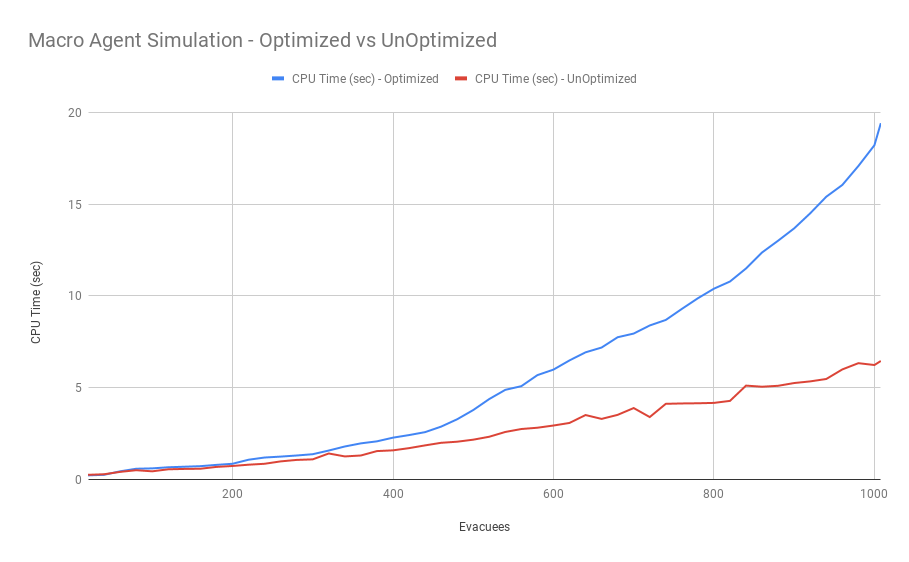
\includegraphics[scale=0.5]{simulation/Macro_Agent_Simulation.png}
  \caption{Macro Agent Simulation - Optimized vs UnOptimized Algorithms}
  \label{Macro Agent Simulation}
\end{figure}

The above figure \ref{Macro Agent Simulation} depicts the difference in the performance experienced as the constraints placed are higher in count and complexity. In the present scenario, not all the constraints are incorporated however. In macro agent simulation, no grouping is employed, hence there is no grouping constraint. This in turn also affects the varying speed constraint as groups of agents are not involved. It is also noteworthy mentioning that single agents can be considered as individual groups as well. Since there is no such constraint, the average of 1.2 $m/s$ velocity for all agents is applied and the simulation of the agents are then performed.


\subsection{Case 2: Run Time Comparison between Micro and Macro Agent Simulation}
\label{sec: Case 2: Run Time Comparison between Micro and Macro Agent Simulation}

This case is similar in terms of objective to the previous case \ref{sec: Case 1: Macro Agent Simulation Comparing Optimized and Un-Optimized Algorithms}. However the key difference lies in what is compared in this particular scenario. Micro and macro agent simulation scenarios are compared in this case. Since there is micro agents that are also included, grouping constraints are included and subsequently varying velocities based on grouping and affiliation.

According to the work by Wagnild et al. \cite{ref24}, walking speeds are highly depend on the company and the lowest speed of the person present in the group. This scenario is inclusive of group constraints. However this scenario is also only to compare the actual running times of the simulated output. Complexities regarding group dynamics are not compared here. To keep the results coherent, the macro agents are considered with the uniform speed as mentioned in the previous section. The micro agents consists of mixed groups and individuals. To keep group velocity diversity among the micro agents, 20\% of the total number of micro agents are randomly distributed with varying speeds between the range of 0.7 $m/s$ and 1.5 $m/s$.   

The comparison values are based off on the pessimistic path scenario as presented in \cite{ref5}. A cross way comparison between macro agents with un-optimized algorithm, macro agents simulated with optimized algorithm and micro agent with constraints is tabulated in the table below. The CPU run time values for the microscopic agents that are simulated using the un-optimzed are obtained from the charted values from table 2.0 from the aforementioned paper, based on which the other two comparisons can be made and analyzed.

A total number of evacuees upto 1008 are considered for the comparisons, similar to the previous section \ref{sec: Case 1: Macro Agent Simulation Comparing Optimized and Un-Optimized Algorithms}. 

\begin{table}
\centering
\begin{adjustbox}{angle=270}
\scalebox{0.7}{
\begin{tabular}{|l|l|l|l|} 
\hline
Evacuees & CPU Time (sec) - Micro Agent Sim:Optimized with Constraints & Evacuees & CPU Time (sec) - Micro Agent Sim:Optimized with Constraints  \\ 
\hline
20       & 0.4                                                         & 540      & 10.8                                                         \\
40       & 0.46                                                        & 560      & 11.5                                                         \\
60       & 0.6                                                         & 580      & 12.3                                                         \\
80       & 0.8                                                         & 600      & 13.8                                                         \\
100      & 0.9                                                         & 620      & 14.97                                                        \\
120      & 1.01                                                        & 640      & 15.92                                                        \\
140      & 1.11                                                        & 660      & 17.3                                                         \\
160      & 1.4                                                         & 680      & 19.2                                                         \\
180      & 1.7                                                         & 700      & 21.84                                                        \\
200      & 2                                                           & 720      & 23.7                                                         \\
220      & 2.3                                                         & 740      & 25.9                                                         \\
240      & 2.4                                                         & 760      & 27.9                                                         \\
260      & 2.7                                                         & 780      & 30.2                                                         \\
280      & 3.2                                                         & 800      & 33.5                                                         \\
300      & 3.5                                                         & 820      & 36.7                                                         \\
320      & 3.9                                                         & 840      & 39                                                           \\
340      & 4.3                                                         & 860      & 43.3                                                         \\
360      & 4.8                                                         & 880      & 47.2                                                         \\
380      & 5.4                                                         & 900      & 50.34                                                        \\
400      & 5.9                                                         & 920      & 54.2                                                         \\
420      & 6.5                                                         & 940      & 58.99                                                        \\
440      & 6.97                                                        & 960      & 64.2                                                         \\
460      & 7.6                                                         & 980      & 68.2                                                         \\
480      & 8.1                                                         & 1000     & 74.78                                                        \\
500      & 8.7                                                         & 1008     & 76.34                                                        \\
520      & 9.7                                                         &          &                                                              \\
\hline
\end{tabular}}
\end{adjustbox}
\caption{CPU Time Comparison between Micro and Macro Agent Simulation}
\label{CPU Time Comparison between Micro and Macro Agent Simulation}
\end{table}  

As it can be noted from the above table \ref{CPU Time Comparison between Micro and Macro Agent Simulation}, the time taken for the micro agent simulation far exceeds the time taken by both the previous simulations - for macro agent using both optimized and un-optimized algorithms. However, it should be noted that the micro agent simulation has 20\% of the entire participants at a reduced movement speed, during each simulation run. Since the number of reduced movement speed agents increase exponentially for each trial run, so does the computation time. These agents who have reduced speeds are also randomized to form certain affliate bonds and groups. 

More discussion on the nature of such groups and their implications are discussed in the next sub-section where the evacuation time is discussed in detail and simulations are run in order to observe the actual time taken due to the additional constraints.

The below figure \ref{Micro vs Macro Agent Simulation} represents the comparison between the 3 major simulation models and their exceedingly apparent ranges of computation times. 

\begin{figure}[H]
  \centering
  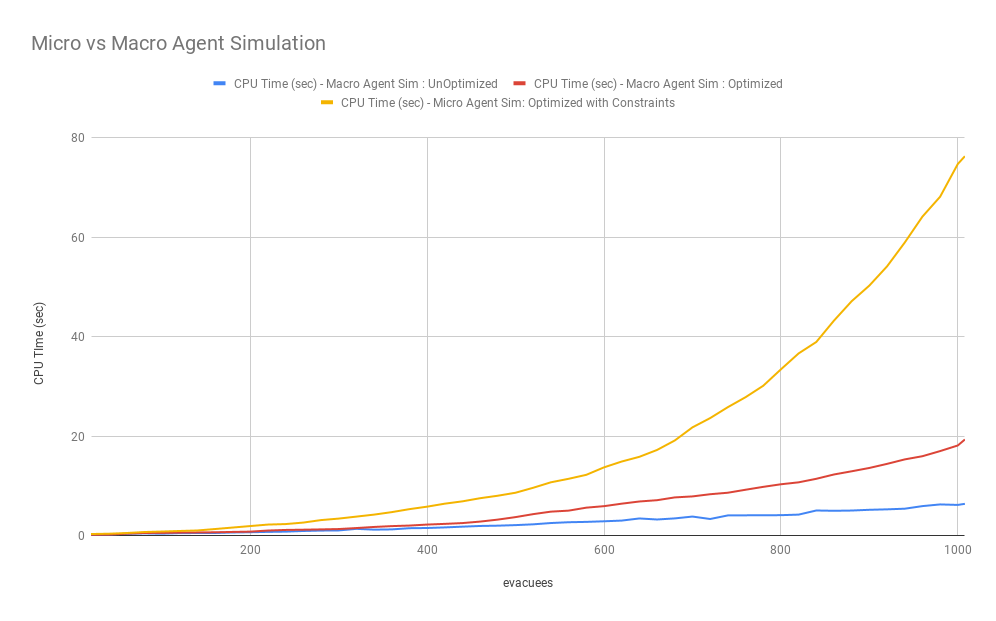
\includegraphics[scale=0.47]{simulation/Micro_vs_Macro_Agent_Simulation.png}
  \caption{Micro vs Macro Agent Simulation}
  \label{Micro vs Macro Agent Simulation}
\end{figure}

From the figure, the following inferences can be made:

\begin{enumerate}
  \item The macro agent simulation with no constraints and simulated according to the base algorithm and a constant $v_{max}$ movement velocity has a time complexity of $O(N)$.
  \item The macro agent simulation subjected to constraints such as social force definition, area capacity and flow capacity, exhibit a time complexity of $O(N^2)$.
  \item Micro agent simulation subjected to varying speeds and grouping in addition to social forces and flow capacity definition for congestion control, exhibit a time complexity of $O(N^3)$.
\end{enumerate}

The implications for these inferences will be discussed in section 4.3.


\subsection{Case 3: Congestion Dynamics and Flow Control}
\label{sec: Case 3: Congestion Dynamics and Flow Control}

This section presents a detailed case on the effect of the width of emergency exits on the evacuation time. 


The following table \ref{Emergency Exits Width vs Evacuation Time : Optimistic Values for Macro} depicts optimistic values for macro agents whilst varying exit capacities and thus in turn affecting flow dynamics.

\begin{table}[H]
\centering
\scalebox{0.7}{
\begin{tabular}{|l|l|l|} 
\hline
Emergency Exit Width (m) & \begin{tabular}[c]{@{}l@{}}Evacuation Time Horizon $(\tau)$ - \\Optimistic values for Unoptimized Algorithm\end{tabular} & \begin{tabular}[c]{@{}l@{}}Evacuation Time Horizon $(\tau)$ - \\Optimistic Values for Optimized Algorithm\end{tabular}  \\ 
\hline
0.4                      & 45                                                                                                                  & 83                                                                                                                 \\
0.5                      & 43                                                                                                                  & 79                                                                                                                 \\
0.6                      & 37                                                                                                                  & 76                                                                                                                 \\
0.7                      & 33                                                                                                                  & 73                                                                                                                 \\
0.8                      & 28                                                                                                                  & 70                                                                                                                 \\
0.9                      & 25                                                                                                                  & 68                                                                                                                 \\
1.0                      & 22                                                                                                                  & 62                                                                                                                 \\
1.1                      & 20                                                                                                                  & 58                                                                                                                 \\
1.2                      & 16                                                                                                                  & 53                                                                                                                 \\
1.3                      & 12                                                                                                                  & 48                                                                                                                 \\
1.4                      & 11                                                                                                                  & 45                                                                                                                 \\
1.5                      & 10                                                                                                                  & 40                                                                                                                 \\
1.6                      & 9                                                                                                                   & 37                                                                                                                 \\
1.7                      & 9                                                                                                                   & 32                                                                                                                 \\
1.8                      & 8                                                                                                                   & 29                                                                                                                 \\
1.9                      & 7                                                                                                                   & 25                                                                                                                 \\
2.0                      & 6                                                                                                                   & 20                                                                                                                 \\
2.1                      & 5                                                                                                                   & 18                                                                                                                 \\
2.2                      & 5                                                                                                                   & 15                                                                                                                 \\
2.3                      & 5                                                                                                                   & 12                                                                                                                 \\
2.4                      & 4                                                                                                                   & 8                                                                                                                  \\
2.5                      & 3                                                                                                                   & 6                                                                                                                  \\
2.6                      & 3                                                                                                                   & 5                                                                                                                  \\
2.7                      & 3                                                                                                                   & 3                                                                                                                  \\
2.8                      & 2                                                                                                                   & 2                                                                                                                  \\
2.9                      & 2                                                                                                                   & 2                                                                                                                  \\
3.0                      & 1                                                                                                                   & 1                                                                                                                  \\
\hline
\end{tabular}}
\caption{Emergency Exits Width vs Evacuation Time : Optimistic Values for Macro}
\label{Emergency Exits Width vs Evacuation Time : Optimistic Values for Macro}
\end{table}

\begin{table}[H]
\centering
\scalebox{0.7}{
\begin{tabular}{|l|l|l|} 
\hline
    Emergency Exit Width (m) & \begin{tabular}[c]{@{}l@{}}Evacuation Time Horizon $(\tau)$ -\\Pessimistic Values for UnOptimized Algorithm\end{tabular} & \begin{tabular}[c]{@{}l@{}}Evacuation Time Horizon $(\tau)$ -\\Pessimistic Values for Optimized Algorithm\end{tabular}  \\ 
\hline
0.4                      & 120                                                                                                                 & 205                                                                                                                \\
0.5                      & 105                                                                                                                 & 192                                                                                                                \\
0.6                      & 94                                                                                                                  & 181                                                                                                                \\
0.7                      & 86                                                                                                                  & 173                                                                                                                \\
0.8                      & 76                                                                                                                  & 163                                                                                                                \\
0.9                      & 68                                                                                                                  & 155                                                                                                                \\
1.0                      & 62                                                                                                                  & 140                                                                                                                \\
1.1                      & 56                                                                                                                  & 127                                                                                                                \\
1.2                      & 53                                                                                                                  & 111                                                                                                                \\
1.3                      & 48                                                                                                                  & 101                                                                                                                \\
1.4                      & 45                                                                                                                  & 93                                                                                                                 \\
1.5                      & 42                                                                                                                  & 80                                                                                                                 \\
1.6                      & 37                                                                                                                  & 72                                                                                                                 \\
1.7                      & 33                                                                                                                  & 65                                                                                                                 \\
1.8                      & 29                                                                                                                  & 52                                                                                                                 \\
1.9                      & 25                                                                                                                  & 47                                                                                                                 \\
2.0                      & 20                                                                                                                  & 30                                                                                                                 \\
2.1                      & 18                                                                                                                  & 19                                                                                                                 \\
2.2                      & 15                                                                                                                  & 17                                                                                                                 \\
2.3                      & 12                                                                                                                  & 14                                                                                                                 \\
2.4                      & 8                                                                                                                   & 11                                                                                                                 \\
2.5                      & 6                                                                                                                   & 8                                                                                                                  \\
2.6                      & 5                                                                                                                   & 6                                                                                                                  \\
2.7                      & 3                                                                                                                   & 5                                                                                                                  \\
2.8                      & 2                                                                                                                   & 3                                                                                                                  \\
2.9                      & 2                                                                                                                   & 2                                                                                                                  \\
3.0                      & 1                                                                                                                   & 1                                                                                                                  \\
\hline
\end{tabular}}
\caption{Emergency Exits Width vs Evacuation Time : Pessimistic values for Macro Agent Simulation}
\label{Emergency Exits Width vs Evacuation Time : Pessimistic values for Macro Agent Simulation}
\end{table}



\begin{table}[H]
\centering
\scalebox{0.7}{
\begin{tabular}{|l|l|l|} 
\hline
Emergency Exit Width (m) & \begin{tabular}[c]{@{}l@{}}Evacuation Time Horizon $(\tau)$ - \\Optimistic Values for Micro Agent Simulation\end{tabular} & \begin{tabular}[c]{@{}l@{}}Evacuation Time Horizon $(\tau)$ - \\Pessimistic Values for Micro Agent Simulation\end{tabular}  \\ 
\hline
0.4                      & 246                                                                                                                  & 415                                                                                                                    \\
0.5                      & 223                                                                                                                  & 370                                                                                                                    \\
0.6                      & 202                                                                                                                  & 340                                                                                                                    \\
0.7                      & 192                                                                                                                  & 306                                                                                                                    \\
0.8                      & 184                                                                                                                  & 292                                                                                                                    \\
0.9                      & 178                                                                                                                  & 270                                                                                                                    \\
1.0                      & 155                                                                                                                  & 240                                                                                                                    \\
1.1                      & 140                                                                                                                  & 212                                                                                                                    \\
1.2                      & 129                                                                                                                  & 193                                                                                                                    \\
1.3                      & 111                                                                                                                  & 163                                                                                                                    \\
1.4                      & 101                                                                                                                  & 140                                                                                                                    \\
1.5                      & 85                                                                                                                   & 124                                                                                                                    \\
1.6                      & 74                                                                                                                   & 112                                                                                                                    \\
1.7                      & 65                                                                                                                   & 99                                                                                                                     \\
1.8                      & 51                                                                                                                   & 83                                                                                                                     \\
1.9                      & 48                                                                                                                   & 60                                                                                                                     \\
2.0                      & 31                                                                                                                   & 47                                                                                                                     \\
2.1                      & 19                                                                                                                   & 33                                                                                                                     \\
2.2                      & 16                                                                                                                   & 28                                                                                                                     \\
2.3                      & 13                                                                                                                   & 20                                                                                                                     \\
2.4                      & 10                                                                                                                   & 16                                                                                                                     \\
2.5                      & 8                                                                                                                    & 9                                                                                                                      \\
2.6                      & 7                                                                                                                    & 8                                                                                                                      \\
2.7                      & 5                                                                                                                    & 6                                                                                                                      \\
2.8                      & 3                                                                                                                    & 3                                                                                                                      \\
2.9                      & 2                                                                                                                    & 2                                                                                                                      \\
3.0                      & 1                                                                                                                    & 1                                                                                                                      \\
\hline
\end{tabular}}
\caption{Emergency Exits Width vs Evacuation Time : Micro Agent Simulation}
\label{Emergency Exits Width vs Evacuation Time : Micro Agent Simulation}
\end{table}

\begin{figure}[H]
  \centering
  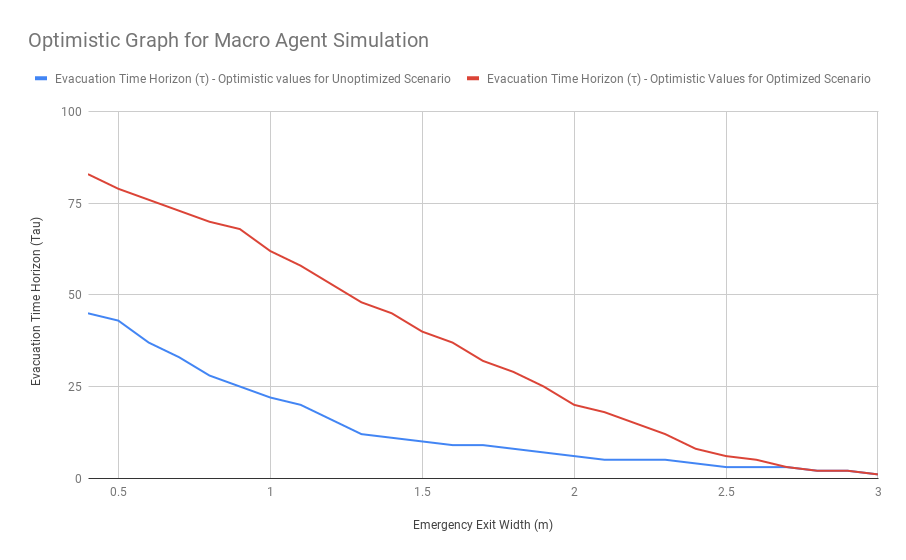
\includegraphics[scale=0.5]{simulation/Optimistic_Graph_for_Macro_Agent_Simulation.png}
  \caption{Optimistic Graph for Macro Agent Simulation}
  \label{Optimistic Graph for Macro Agent Simulation}
\end{figure}

\begin{figure}[H]
  \centering
  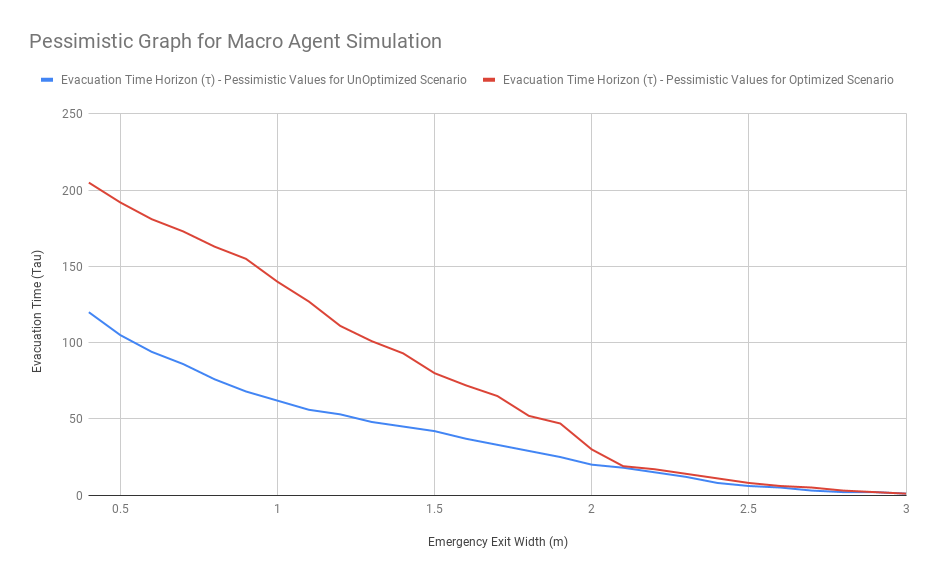
\includegraphics[scale=0.5]{simulation/Pessimistic_Graph_for_Macro_Agent_Simulation.png}
  \caption{Pessimistic Graph for Macro Agent Simulation}
  \label{Pessimistic Graph for Macro Agent Simulation}
\end{figure}

\begin{figure}[H]
  \centering
  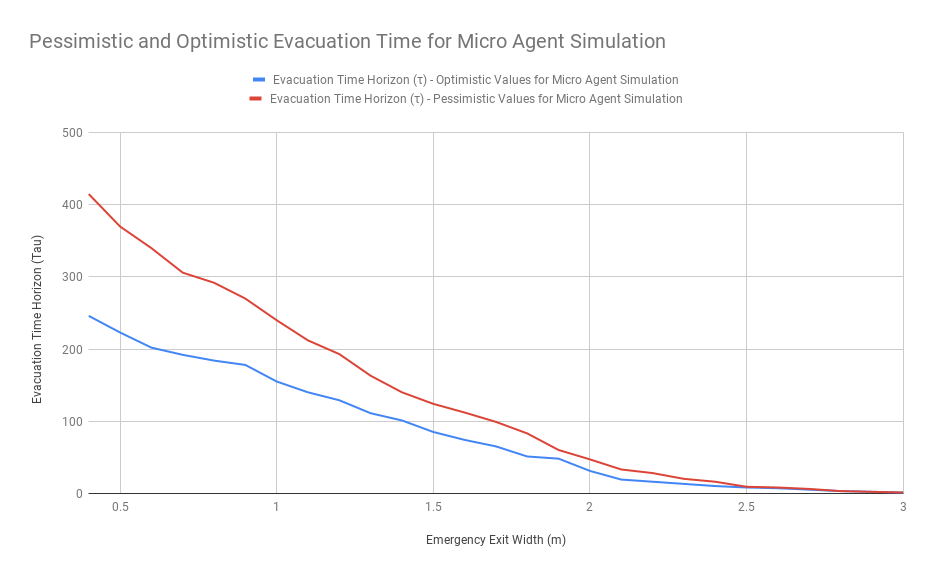
\includegraphics[scale=0.5]{simulation/Pessimistic_and_Optimistic_Evacuation_Time_for_Micro_Agent_Simulation.png}
  \caption{Pessimistic and Optimistic Evacuation Time for Micro Agent Simulation}
  \label{Pessimistic and Optimistic Evacuation Time for Micro Agent Simulation}
\end{figure}

\begin{figure}[H]
  \centering
  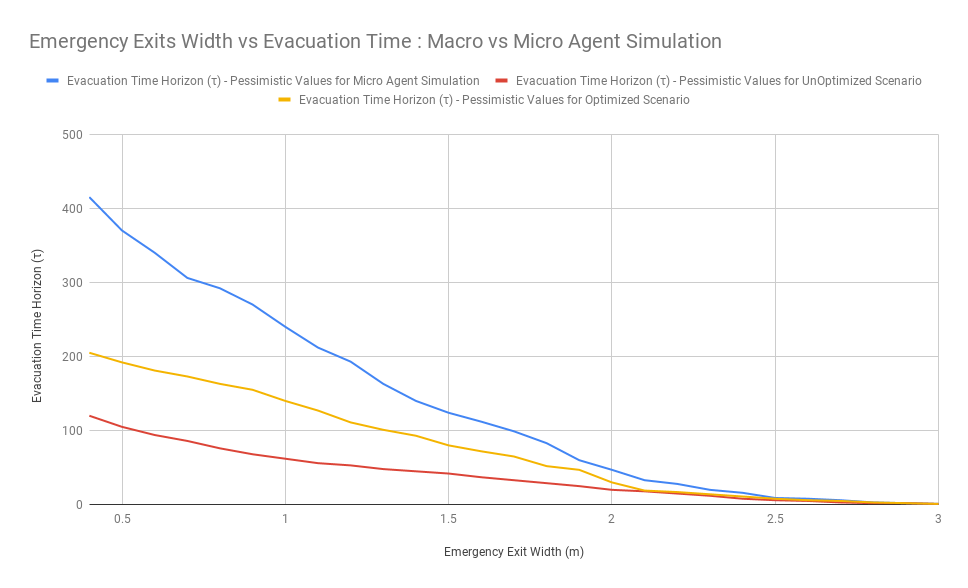
\includegraphics[scale=0.5]{simulation/summary.png}
  \caption{Emergency Exits Width vs Evacuation Time : Macro vs Micro Agent Simulation}
  \label{Emergency Exits Width vs Evacuation Time : Macro vs Micro Agent Simulation}
\end{figure}